\documentclass[letterpaper,12pt]{article}
% packages used
    \usepackage{natbib}
	\usepackage{threeparttable}
	\usepackage[format=hang,font=normalsize,labelfont=bf]{caption}
	\usepackage{amsmath}
	\usepackage{amssymb}
	\usepackage{amsthm}
	\usepackage{caption}
	\usepackage{subcaption}
	\usepackage{setspace}
	\usepackage{float,color}
	\usepackage[pdftex]{graphicx}
	\usepackage{hyperref}
	\usepackage{multirow}
	\usepackage{float,graphicx,color}
	\usepackage{graphics}
    \usepackage{placeins}
    \usepackage{authblk}
    \usepackage{tikz}

% other setup
	\hypersetup{colorlinks, linkcolor=red, urlcolor=blue, citecolor=red, hypertexnames=false}
	\graphicspath{{./figures/}}
	\DeclareMathOperator*{\Max}{Max}
	\bibliographystyle{aer}
	\numberwithin{equation}{section}
	\numberwithin{figure}{section}
	\numberwithin{table}{section}
	\newcommand\ve{\varepsilon}


\begin{document}

\begin{titlepage}
	\title{Playing the Lottery: Even When It's a Good Deal, It's Not}
    
    \thanks{The views expressed in this paper are the authors' and should not be interpreted as those of the Congressional Budget Office.}

	\author{Kerk L. Phillips \\
	\small US Congressional Budget Office \\
	\small \href{mailto:kerk.phillips@cbo.gov}{kerk.phillips@cbo.gov} }


	\date{May 30, 2023\\
	\small{version 2023.05.a}}

	
	\maketitle

	\vspace{-0.3in}
	\begin{abstract}
	\small{
	This paper shows that for many common utility function and distributions of expected income, playing the lottery decreases expected utility even in cases where the expected payoff is greater than the price of a lottery ticket.

	\vspace{0.1in}

	\textit{keywords:} lottery, risk aversion, welfare analysis, numerical analysis

	\vspace{0.1in}

	\textit{JEL classifications: D0, D6, H8} }
	\end{abstract}

	\centering
	Preliminary, Comments Appreciated

	\thispagestyle{empty}
\end{titlepage}

\begin{spacing}{1.5}

\section{Introduction} \label{sec_intro}

	As a general rule the expected value of a lottery ticket is less than the price.  This is because the lottery is a money-generation process for the government that runs it and revenue inflows must, on average, exceed the payment outflows.  However, with some lotteries on some occasions, when there is no jackpot winner and the jackpot rolls over for several consecutive weeks, the expected payoff can exceed the price of the ticket.  For example, the odds of matching all the numbers for the weekly Powerball lottery are approximately 292 million to one, while the odds for the MegaMillions lottery are 302 million to one.  The price for both lottery tickets is two dollars.  The average payout for the highest 5 jackpots from these two lotteries is 1.57 billion dollars.  This gives an approximate expected return of \$5.29 on a two-dollar lottery ticket, or an expected return of 164\%.  Even accounting for the fact that the present values of jackpots are substantially smaller than the numbers reported, this is still a sizable expected return on an investment.

	In these cases, is it ever worthwhile to purchase a lottery ticket?  On one hand, the odds of winning are overwhelmingly small, and the \$2 cost of the ticket is a virtually guaranteed loss.  On the other hand, in the that one-in-300 million case the payout is worth more than a billion dollars.  Which of these two dominates in expected utility terms?  Not surprisingly, the answer depends on the purchaser's risk aversion.  A risk-neutral purchaser would clearly be better off purchasing the ticket.  However, most people are risk averse to some degree or another.  In this paper I show that for a wide ranges of parameterized utility functions, there is a net loss in expected utility when purchasing a lottery ticket.  This result is quite intuitive as it is hard to think of an asset purchase that introduced more risk that a lottery ticket.  By comparison, the odds of being killed by lightning over the course of a lifetime in the U.S. are one in 153,000, or a little over 11 million to one in a given year.  In order for a lottery ticket to generate gains in expected utility, risk aversion must be unreasonably small, or the the odds of winning must be unreasonably high.

\section{Numerical Analysis} \label{sec_numer}

	In this section we calculate the expected welfare loss or gain from playing the lottery.  We assume that a lottery player already has a stochastic endowment of non-lottery income, denoted $x$ which will all be spent on consumption or the purchase of a single lottery ticket.  Utility from consumption comes from one of the five functional forms in Section \ref{sec_util}.  The distribution of non-lottery income is described by one of the probability density functions from Section \ref{sec_dist}.  The parameters of the lottery are laid out in Section \ref{sec_lottery}.

	If the individual chooses not to play the lottery, their consumption ($c$) is exactly equal to their stochastic non-lottery income, so $c = x$.  If they choose to play the lottery then with probability $\tfrac{1}{\omega}$ their consumption will be their non-lottery income plus the lottery payoff ($p$) minus the cost of the lottery ticket ($t$), giving $c = x + p - t$.  However, if they lose the lottery, their consumption is non-lottery income minus the cost of the ticket, $c = x - t$

	Disposable income is discretized over a grid with $n$ equally spaced points between $x_{min}$ and $x_{max}$.  The probabilities are generated using the density functions below and are scaled appropriately so that they sum to 1 over the $n$ points in the grid.


	\subsection{Utility Functions} \label{sec_util}

		Constant Relative Risk Aversion (CRRA)
		\begin{equation}
			u(c) = \frac{c^{1-\gamma}-1}{1-\gamma}
		\end{equation}

		Stone-Geary
		\begin{equation}
			u(c) = \frac{(c-\underline{c})^{1-\gamma}-1}{1-\gamma}
		\end{equation}

		Exponential
		\begin{equation}
			u(c) = 1-e^{-a c}
		\end{equation}

		Hyperbolic Absolute Risk Aversion (HARA)
		\begin{equation}
			u(c) = \frac{1-\gamma}{\gamma} \left( \frac{a c}{1-\gamma} + b \right)^\gamma
		\end{equation}

		Logarithmic
		\begin{equation}
			u(c) = \ln c
		\end{equation}

	\subsection{Non-Lottery Income Distributions} \label{sec_dist}

		Beta Probability Density Function
		\begin{equation}
			f(x) = \frac{\left( \frac{x-x_{min}}{x_{max}-x_{min}} \right)^{a-1} \left(1 - \frac{x-x_{min}}{x_{max}-x_{min}} \right )^{b-1}} {B(a,b)}
		\end{equation}
		where $B(a,b)$ is the beta function.  In this paper $a=2, b=2.2$.

		Normal Probability Density Function
		\begin{equation}
			f(x) = \frac{1}{\sigma \sqrt{2 \pi}} e^{-\frac{1}{2} \left(\frac{x-\mu}{\sigma} \right)^2}
		\end{equation}
		where $\mu = \frac{x_{max}+x_{min}}{2}, \sigma = \frac{x_{max}-x_{min}}{3}$.

		Uniform Probability Density Function
		\begin{equation}
			f(x) = q = \frac{1}{n}
		\end{equation}	

	\subsection{Lottery Setup} \label{sec_lottery}

		There are two lotteries considered in this paper.  First, a typical lottery with payouts in line with those found for the Powerball lottery.  And second, a lottery with a very large payout in line with the highest history jackpots for the Powerball and MegaMillions lotteries.

		For a typical lottery, a ticket costs 2 dollars and pays \$226 million with odds of 1:300,000,000.  This gives a expected net return of -62.3 percent, with a ticket paying an expected value of 75 cents.

		A high payout lottery has the same odds and ticket cost, pays \$ 1.5 billion.  This gives a expected net return of 150 percent, with a ticket paying an expected value of 5 dollars.

\section{Results} \label{sec_results}

	I first run a set of calculations using a grid for $x$ with $n=101$, $x_{min} = 20,000$ and $x_{max} = 150,000$.  This corresponds to an individual with an expected non-lottery income between $70,000$ and $85,000$, but high variance in that income.  I set the payoff in this case to the average jackpot for the Powerball between May 2022 and May 2023, which is 226 million dollars.  In this case the expected change in consumption from playing the lottery is -\$1.25.

	I then run a set of calculations using the same grid, utility, and distribution assumptions as above, but increase the payoff to 1.5 billion dollars, the rough average of the highest five MegaMillions and Powerball payoffs  In every case expected consumption rises by three dollars despite a drop in two dollars due to the cost of a lottery ticket.  However, expected utility falls in every case as well.  The results of these calculations are shown in Table \ref{tab_lottery1} in the fourth column.  For reference, the probability distributions are shown in Figure \ref{fig_PDFs}.  The utility losses from this lottery are virtually the same as playing a typical lottery with an expected consumption loss.  In all cases the expected utility from wining is not sufficiently large to move expected utility in the face of such long odds are wining.  Table \ref{tab_lottery3} shows that the marginal contribution of winning the lottery to expected utility is effectively zero even if the payoff is as high as a years worth of GDP.

	I then set up two alternative individuals.  The first has income between $x_{min} = 20,000$ and $x_{max} = 30,000$ and the second has income between $x_{min} = 140,000$ and $x_{max} = 150,000$.  The results for these two individuals are shown in the last two columns of Table \ref{tab_lottery1}.  The probabilities in these cases are scaled versions of the ones in Figure \ref{fig_PDFs}, having the same shape, but different upper and lower bounds on non-lottery income.

	Table \ref{tab_lottery1} shows that even though expected consumption rises by three dollars for all participants regardless of their utility function or the distribution of their non-lottery income, their expected utility falls.  It also shows that the loss of utility is much greater for low-income individuals than high-income.  The ratio of expected utility lose for low-income to high-income is lowest at 2.45 for HARA utility and a uniform distribution of income, and highest at 1.304E+52 for exponential utility and a beta distribution.

	It is not necessarily the case that expected utility will always be negative from playing the lottery.  If risk aversion were low enough or the odds were good enough then expected utility could rise.  However, as Tables \ref{tab_lottery3} and \ref{tab_lottery4} show, the levels of risk aversion must be unreasonably low, and the odds must be extremely high.  Table \ref{tab_lottery3} calculates the values of $\gamma$, the coefficient of risk aversion, in the CRRA and Stone-Geary utility functions, that will make the high-variance individual indifferent between playing and not playing the lottery.  These values cluster around 0.1.  Most empirical estimates of consumer relative risk aversion range from 1.0 to 4.0 or higher.  Table \ref{tab_lottery4} calculates the odds that will make the high-variance individual indifferent between playing and not playing the lottery for the same utility functions and distributions.  It also shows the expected percent returns on a lottery ticket for these odds.  These are in the range of 228 thousand to 569 thousand percent, numbers which are simply impossible.


	\begin{table}[ht] 
		\caption{Changes in Utility with High Variance}
		\label{tab_lottery1}
		\centering
		\footnotesize
		\begin{tabular}{|lll|lll|}
			\hline
			$u(c)$ & $f(x)$ & Typical & \multicolumn{3}{c}{High Payoff} \\
			& & Payoff & High Variance & Low Income & High Income \\
			\hline
			CRRA & beta & -6.19E-10 & -6.19E-10 & -3.54E-09 & -9.65E-11 \\
			CRRA & normal & -8.43E-10 & -8.43E-10 & -4.30E-09 & -1.02E-10 \\
			CRRA & uniform & -6.86E-10 & -6.86E-10 & -3.34E-09 & -9.52E-11 \\
			\hline
			S-G & beta & -1.09E-09 & -1.09E-09 & -1.08E-08 & -1.11E-10 \\
			S-G & normal & -1.84E-09 & -1.84E-09 & -1.52E-08 & -1.18E-10 \\
			S-G & uniform & -1.52E-09 & -1.52E-09 & -1.00E-08 & -1.10E-10 \\
			\hline
			exponential & beta & -2.46E-15 & -2.46E-15 & -3.27E-13 & -2.51E-65 \\
			exponential & normal & -6.07E-14 & -6.07E-14 & -1.45E-12 & -2.65E-64 \\
			exponential & uniform & -5.62E-14 & -5.62E-14 & -4.30E-13 & -3.30E-65 \\
			\hline
			HARA & beta & -5.51E-03 & -5.45E-03 & -8.97E-03 & -3.63E-03 \\
			HARA & normal & -5.76E-03 & -5.71E-03 & -9.41E-03 & -3.68E-03 \\
			HARA & uniform & -5.30E-03 & -5.25E-03 & -8.81E-03 & -3.62E-03 \\
			\hline
			log & beta & -3.23E-05 & -3.23E-05 & -8.39E-05 & -1.39E-05 \\
			log & normal & -3.62E-05 & -3.62E-05 & -9.25E-05 & -1.43E-05 \\
			log & uniform & -3.13E-05 & -3.13E-05 & -8.11E-05 & -1.38E-05 \\
			\hline
		\end{tabular}
	\end{table}

	\begin{figure}[ht] 
		\centering
		\caption{Three Probability Distributions}
		\label{fig_PDFs}
		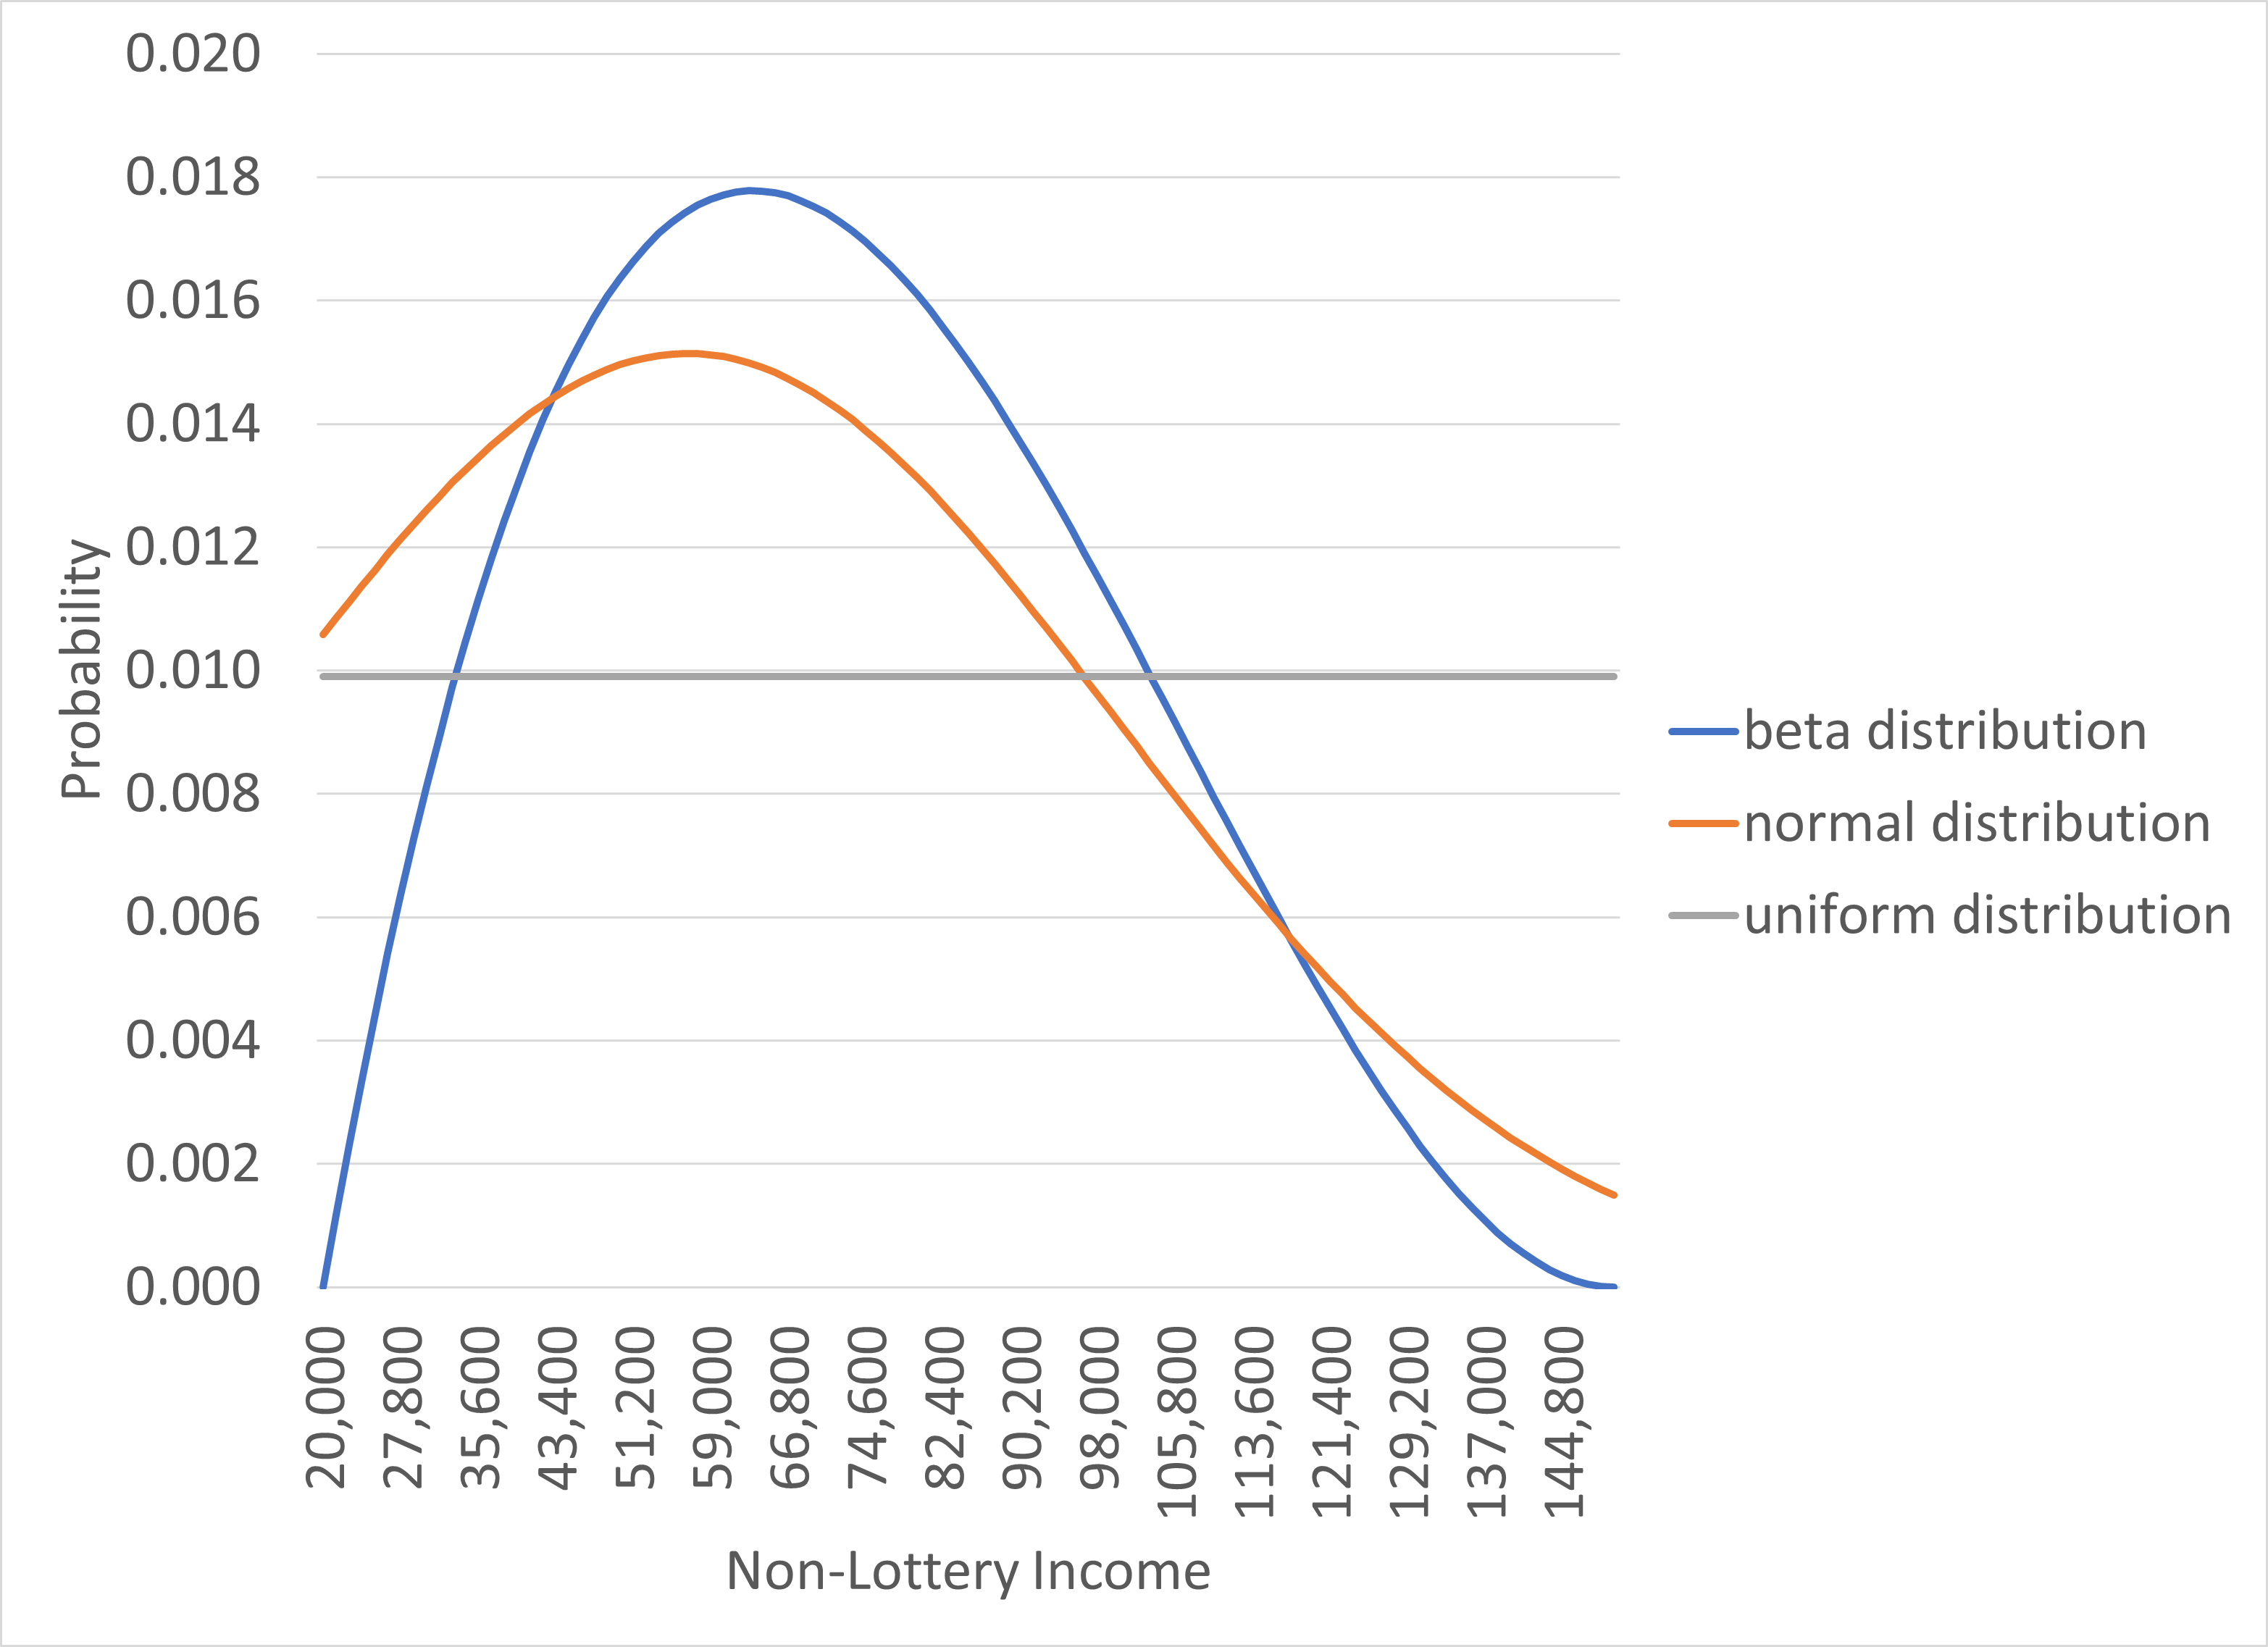
\includegraphics[width=.9\textwidth]{images/PDFs.png}
	\end{figure}


	\begin{table}[ht] 
		\caption{Decomposition of Expected Utility from Playing the Lottery}
		\label{tab_lottery2}
		\centering
		\small
		\begin{tabular}{|ll|lll|}
			\hline
			Payoff & Utility & EU from losing  & EU from Winning & EUwin/EUlose \\
			\hline
			226 million & CRRA & 0.99998 & 3.3333E-09 & 0.0000003333\% \\
			226 million & S-G & 0.99998 & 3.3333E-09 & 0.0000003333\% \\
			226 million & exponential & 1.00000 & 3.3333E-09 & 0.0000003333\% \\
			226 million & HARA & 10007.19736 & 7.8326E-05 & 0.0000007827\% \\
			226 million & log & 11.11323 & 6.4121E-08 & 0.0000005770\% \\
			1.5 billion & CRRA & 0.99998 & 3.3333E-09 & 0.0000003333\% \\
			1.5 billion & S-G & 0.99998 & 3.3333E-09 & 0.0000003333\% \\
			1.5 billion & exponential & 1.00000 & 3.3333E-09 & 0.0000003333\% \\
			1.5 billion & HARA & 10007.19736 & 1.8560E-04 & 0.0000018546\% \\
			1.5 billion & log & 11.11323 & 7.0429E-08 & 0.0000006337\% \\
			23.3 trillion & CRRA & 0.99998 & 3.3333E-09 & 0.0000003333\% \\
			23.3 trillion & S-G & 0.99998 & 3.3333E-09 & 0.0000003333\% \\
			23.3 trillion & exponential & 1.00000 & 3.3333E-09 & 0.0000003333\% \\
			23.3 trillion & HARA & 10007.19736 & 2.2706E-02 & 0.0002268954\% \\
			23.3 trillion & log & 11.11323 & 1.0258E-07 & 0.0000009231\% \\
			\hline
		\end{tabular}
	\end{table}


	\begin{table}[ht] 
		\caption{Values of $\gamma$ That Make the Change in Utility Equal Zero}
		\label{tab_lottery3}
		\centering
		\begin{tabular}{|l|ll|}
		    \hline
			$f(x)$ & CRRA & S-G \\
			\hline
			beta & 0.1022 & 0.1001 \\
			normal & 0.1013 & 0.0990 \\
			uniform & 0.1033 & 0.1011 \\
			\hline
		\end{tabular}
	\end{table}

	\begin{table}[ht] 
		\caption{Odds That Make the Change in Utility Equal Zero}
		\label{tab_lottery4}
		\centering
		\begin{tabular}{|l|ll|ll|}
		    \hline
			$f(x)$ & \multicolumn{2}{c}{CRRA} & \multicolumn{2}{c}{S-G} \\
			& odds & return & odds & return \\
			\hline
			beta & 1:26000 & 288462\% & 1:18600 & 403226\% \\
			normal & 1:21500 & 348837\% & 1:13200 & 568182\% \\
			uniform & 1:22700 & 330396\% & 1:13600 & 551471\% \\
			\hline
		\end{tabular}
	\end{table}


\FloatBarrier

\section{Conclusions} \label{sec_concl}

	This paper has demonstrated that buying a lottery ticket reduces expected utility for a wide range of utility functions and reasonable levels of risk aversion.  The only cases when expected utility can rise is when the expected payoff from a lottery ticket exceeds the price of the ticket, which occurs only rarely when the jackpot rolls over several times in a row due to no winning number being drawn.  Even in this case, for expected utility to rise, the individual must be essentially risk neutral.
	

%\newpage
%\nocite{*}
%\bibliography{Lottery}

\end{spacing}

\end{document}